% Landmark generation by relaxed reachability, and why the count is not a bound.
\documentclass[tikz,border=0pt]{standalone}
\usepackage{tikz}
\usepackage[normalem]{ulem}
\usetikzlibrary{backgrounds,arrows.meta,positioning}
\definecolor{hdblue}{HTML}{1B4F8A}
\definecolor{hdred}{HTML}{A62B1F}
\begin{document}
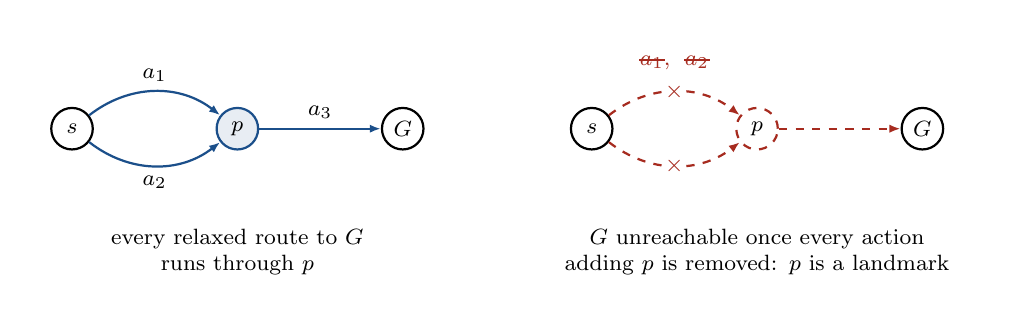
\begin{tikzpicture}[
    show background rectangle, inner frame sep=7pt,
    background rectangle/.style={fill=white},
    font=\footnotesize, >={Latex[length=4pt]},
    fact/.style={circle,draw=black,thick,fill=white,minimum size=15pt,inner sep=0pt},
    lm/.style={circle,draw=hdblue,thick,fill=hdblue!10,minimum size=15pt,inner sep=0pt},
    gone/.style={circle,draw=hdred,thick,dashed,fill=white,minimum size=15pt,inner sep=0pt},
    edge/.style={->,hdblue,thick},
    dead/.style={->,hdred,thick,dashed}]

  % ---- panel A: p is on every relaxed route to the goal
  \begin{scope}
    \node[fact] (s)  at (0,0)      {$s$};
    \node[lm]   (p)  at (2.1,0)    {$p$};
    \node[fact] (g)  at (4.2,0)    {$G$};
    \draw[edge] (s) to[bend left=38]  node[above,black] {$a_1$} (p);
    \draw[edge] (s) to[bend right=38] node[below,black] {$a_2$} (p);
    \draw[edge] (p) -- node[above,black] {$a_3$} (g);
    \node[anchor=north,align=center,text width=4.6cm] at (2.1,-1.15)
         {every relaxed route to $G$\\ runs through $p$};
  \end{scope}

  % ---- panel B: remove every action adding p
  \begin{scope}[xshift=6.6cm]
    \node[fact] (s2) at (0,0)   {$s$};
    \node[gone] (p2) at (2.1,0) {$p$};
    \node[fact] (g2) at (4.2,0) {$G$};
    \draw[dead] (s2) to[bend left=38]
      node[pos=0.5,hdred,fill=white,inner sep=1pt] {$\times$} (p2);
    \draw[dead] (s2) to[bend right=38]
      node[pos=0.5,hdred,fill=white,inner sep=1pt] {$\times$} (p2);
    \draw[dead] (p2) -- (g2);
    \node[anchor=south,hdred] at (1.05,0.62) {\sout{$a_1$},\; \sout{$a_2$}};
    \node[anchor=north,align=center,text width=5.2cm] at (2.1,-1.15)
         {$G$ unreachable once every action\\ adding $p$ is removed: $p$ is a landmark};
  \end{scope}
\end{tikzpicture}
\end{document}
